% Provenance (never printed): see sources/outline_sources.md (Year 1: crystal
% chemistry of minerals, silicates, solid solutions, mineral formulas, the main
% rock-forming minerals). Olivine curves in figdata/bachelor-1/solid_solution.py;
% the olivine analysis of the problem is invented (Fo about 82); exercise and
% problem values in the Book 3 scratch calculator calc/ch07.py.
\chapter{造岩矿物}\label{ch:b1:rock-forming-minerals}

一块花岗岩台面上可见三四种颗粒：玻璃质的灰色石英、粉红色
或白色的\omterm{def:b1:rock-forming-minerals:groups}{长石}、黑色的\omterm{def:b1:rock-forming-minerals:groups}{云母}片。海滩上的沙几乎全是石英。
散落在玄武岩中的绿色小晶体是\omterm{def:b1:rock-forming-minerals:groups}{橄榄石}，同一种
\omterm{def:b1:rock-forming-minerals:mineral}{矿物}（成分略有不同）构成了上
地幔的大部分。少数几种\omterm{def:b1:rock-forming-minerals:mineral}{矿物}几乎构成了所有岩石，其中
几乎全部是硅酸盐：氧和硅是地壳中
最丰富的两种元素，它们结合成四面体，以少数简单方式相连。本章
说明连接方式如何决定硅酸盐的化学式和晶习，
一种元素如何替代晶体中的另一种元素，使\omterm{def:b1:rock-forming-minerals:mineral}{矿物}成为一个
成分范围而非单一成分，化学分析如何化为化学式，以及
主要造岩\omterm{def:b1:rock-forming-minerals:mineral}{矿物}是什么。全章以一块玄武岩中的\omterm{def:b1:rock-forming-minerals:groups}{橄榄石}作结，
对其进行分析、重新计算并称重。

\begin{recall}
晶体是原子在晶格上周期性重复排列的固体；晶胞是
最小的重复单元，离子的配位数即其
异号电荷的最近邻数目（化学，本科一年级）。离子
半径取决于电荷和配位数。\omterm{def:b1:rock-forming-minerals:mineral}{矿物}可在手标本上
凭借晶习、解理、硬度和光泽加以鉴定（第 2 册，十一年级）。
物质的量以摩尔计，摩尔质量是
一摩尔的质量（化学）。
\end{recall}

\section{什么是矿物}

\begin{definition}[矿物]\label{def:b1:rock-forming-minerals:mineral}
称\emph{矿物}\index{矿物}为天然产出的固体，
具有确定的晶体结构，化学组成固定或
在一定范围内变化。几乎所有矿物都是无机物。
\end{definition}

与之相反，岩石是由一种或几种\omterm{def:b1:rock-forming-minerals:mineral}{矿物}（或玻璃）的
颗粒集合而成的：花岗岩由石英、\omterm{def:b1:rock-forming-minerals:groups}{长石}和\omterm{def:b1:rock-forming-minerals:groups}{云母}组成；石灰岩主要由方解石组成。
定义的两半部分相互独立。窗玻璃具有硅酸盐的
化学组成，却没有晶体结构，因此不是\omterm{def:b1:rock-forming-minerals:mineral}{矿物}，
淬冷熔岩形成的玻璃也不是。反过来，同一化学组成可以
结晶成多种结构，每种结构都是一种不同的
\omterm{def:b1:rock-forming-minerals:mineral}{矿物}。

\begin{definition}[同质多象变体]\label{def:b1:rock-forming-minerals:polymorph}
若两种\omterm{def:b1:rock-forming-minerals:mineral}{矿物}互为\emph{同质多象变体}\index{同质多象变体}，
即二者化学组成相同、晶体结构不同。
\end{definition}

碳可结晶为石墨，它是由六边形网层堆叠而成的结构，
密度为 \qty{2.16}{g.cm^{-3}}；也可结晶为金刚石，骨架中的每个
原子有四个近邻，密度为 \qty{3.51}{g.cm^{-3}}。碳酸钙为
方解石（\qty{2.71}{g.cm^{-3}}）或文石
（\qty{2.93}{g.cm^{-3}}）；二氧化硅为石英（\qty{2.65}{g.cm^{-3}}）或柯石英
（\qty{2.93}{g.cm^{-3}}）；\ce{Al2SiO5} 为蓝晶石（\qty{3.61}{g.cm^{-3}}），
红柱石（\qty{3.15}{g.cm^{-3}}）或夕线石（\qty{3.24}{g.cm^{-3}}）。
% ledger: webmineral:polymorphs, hom:calcite, hom:quartz
在每一对\omterm{def:b1:rock-forming-minerals:polymorph}{同质多象变体}中，密度较大者形成于较高压强下：
在给定温度下，升高压强有利于体积较小的状态
（化学，平衡的移动）。金伯利岩中的金刚石，以及
被陨石撞击的岩石中的柯石英，因此记录了
只有在地幔深部或撞击过程中才能达到的压强。三种
\ce{Al2SiO5} \omterm{def:b1:rock-forming-minerals:polymorph}{同质多象变体}的稳定域在压强–温度平面上彼此划分，
可用于判读变质作用的条件
（本科二年级）。

\section{硅酸盐四面体及其连接方式}

在所有常见硅酸盐中，每个硅原子位于
由四个氧原子占据顶点的正四面体中心：
即化学中已学过的 \ce{SiO4} 单元。硅离子较小，
（四配位时为 \qty{0.26}{\angstrom}），氧离子较大，因此
只能有四个氧原子围绕其排列，不能更多；硅氧键较强，
并部分具有共价性。孤立单元的电荷为 $4 - 4\times2 = -4$。
% ledger: shannon:radii
四面体可以各自独立存在，其电荷由它们之间的金属阳离子平衡，
也可以共用顶点：两个四面体所共有的氧是一个
\emph{桥氧}。两个四面体绝不共用棱或面，否则
两个硅离子会靠得过近。硅酸盐按每个四面体所共用的
顶点数分类（见\cref{def:b1:rock-forming-minerals:silicate-classes}）。

\begin{omfigure}
\tikzset{
  tup/.pic={\filldraw[fill=omLithLime, draw=black, line join=round] (0,0) -- (1,0) -- (0.5,0.866) -- cycle;
            \fill[omThm] (0.5,0.2887) circle (0.11);},
  tdn/.pic={\filldraw[fill=omLithLime, draw=black, line join=round] (0,0) -- (1,0) -- (0.5,-0.866) -- cycle;
            \fill[omThm] (0.5,-0.2887) circle (0.11);},
  linkpanel/.style={x=0.45cm, y=0.45cm, baseline=(current bounding box.south)}}
\setlength{\tabcolsep}{4pt}
\begin{tabular}{cccc}
% (a) the tetrahedron in perspective
\begin{tikzpicture}[linkpanel]
  \useasboundingbox (-1.2,-1.0) rectangle (6.0,4.4);
  \coordinate (T) at (2.2,3.7); \coordinate (L) at (0.3,0.5); \coordinate (R) at (4.1,0.1);
  \coordinate (B) at (3.3,2.1); \coordinate (C) at (2.475,1.6);
  \draw[densely dashed, gray] (L) -- (B) -- (R) (B) -- (T);
  \shade[ball color=omLithShale] (B) circle (0.42);
  \draw[gray] (C) -- (T) (C) -- (L) (C) -- (R) (C) -- (B);
  \shade[ball color=omThm!70] (C) circle (0.24);
  \draw[thick, line join=round] (T) -- (L) -- (R) -- cycle;
  \foreach \p in {T,L,R} \shade[ball color=omLithShale] (\p) circle (0.42);
  \node[right] at (4.5,0.1) {\scriptsize O};
  \node[right] at (2.6,3.8) {\scriptsize O};
  \draw[omThm] (C) -- (4.6,2.2) node[right] {\scriptsize Si};
\end{tikzpicture} &
% (b) nesosilicate: isolated tetrahedra
\begin{tikzpicture}[linkpanel]
  \useasboundingbox (-1.2,-1.0) rectangle (6.0,4.4);
  \pic at (0,0.3) {tup}; \pic at (2.4,0.3) {tup}; \pic at (4.0,1.9) {tdn};
  \pic at (1.2,2.4) {tdn}; \pic at (3.0,2.8) {tup};
\end{tikzpicture} &
% (c) sorosilicate: pairs
\begin{tikzpicture}[linkpanel]
  \useasboundingbox (-1.2,-1.0) rectangle (6.0,4.4);
  \pic at (0,0.9) {tup}; \pic at (1,0.9) {tdn};
  \pic at (2.6,2.6) {tup}; \pic at (3.6,2.6) {tdn};
\end{tikzpicture} &
% (d) cyclosilicate: a ring of six
\begin{tikzpicture}[linkpanel]
  \useasboundingbox (-1.2,-1.0) rectangle (6.0,4.4);
  \begin{scope}[shift={(2.4,1.7)}]
  \foreach \t in {0,60,...,300} {
    \filldraw[fill=omLithLime, draw=black, line join=round] (\t-30:1) -- (\t+30:1) -- (\t:1.732) -- cycle;
    \fill[omThm] (\t:1.155) circle (0.11);}
  \end{scope}
\end{tikzpicture} \\
{\small (a) \ce{SiO4} 四面体} & {\small (b) \omterm{def:b1:rock-forming-minerals:silicate-classes}{岛状硅酸盐}} & {\small (c) \omterm{def:b1:rock-forming-minerals:silicate-classes}{双岛状硅酸盐}} & {\small (d) \omterm{def:b1:rock-forming-minerals:silicate-classes}{环状硅酸盐}} \\
 & {\scriptsize $s = 0$, \ce{SiO4}} & {\scriptsize $s = 1$, \ce{Si2O7}} & {\scriptsize $s = 2$, \ce{Si6O18}} \\[6pt]
% (e) single chain
\begin{tikzpicture}[linkpanel]
  \useasboundingbox (-0.6,-1.2) rectangle (7.6,4.6);
  \begin{scope}[shift={(0,1.5)}]
  \foreach \i in {0,...,3} \pic at (2*\i,0) {tup};
  \foreach \i in {0,...,2} \pic at (2*\i+1,0) {tdn};
  \end{scope}
\end{tikzpicture} &
% (f) double chain: two single chains joined through every other apex
\begin{tikzpicture}[linkpanel]
  \useasboundingbox (-0.6,-1.2) rectangle (7.6,4.6);
  \begin{scope}[shift={(0.5,0.4)}]
  \foreach \i in {0,...,3} {\pic at (2*\i,0) {tup}; \pic at (2*\i,1.732) {tdn};}
  \foreach \i in {0,...,2} {\pic at (2*\i+1,0) {tdn}; \pic at (2*\i+1,1.732) {tup};}
  \end{scope}
\end{tikzpicture} &
% (g) sheet
\begin{tikzpicture}[linkpanel]
  \useasboundingbox (-0.6,-1.2) rectangle (7.6,4.6);
  \foreach \j in {0,1,2} {
    \foreach \i in {0,1,2} {\pic at (2*\i+\j,1.732*\j) {tup};}
    \foreach \i in {0,1} {\pic at (2*\i+\j+1,1.732*\j) {tdn};}}
\end{tikzpicture} &
% (h) framework: a sheet whose apices point alternately up and down
\begin{tikzpicture}[linkpanel]
  \useasboundingbox (-0.6,-1.2) rectangle (7.6,4.6);
  \foreach \j in {0,1,2} {
    \foreach \i in {0,1,2} {\pic at (2*\i+\j,1.732*\j) {tup};}
    \foreach \i in {0,1} {\pic at (2*\i+\j+1,1.732*\j) {tdn};}}
  \foreach \j in {0,1,2} \foreach \i in {0,1} {
    \filldraw[fill=white, draw=omThm, thick] (2*\i+\j+1.5,1.732*\j-0.2887) circle (0.17);}
\end{tikzpicture} \\
{\small (e) 单链} & {\small (f) 双链} & {\small (g) 层状} & {\small (h) 架状} \\
{\scriptsize $s = 2$，\ce{SiO3}} & {\scriptsize $s = 2$ 和 $3$，\ce{Si4O11}} & {\scriptsize $s = 3$，\ce{Si2O5}} & {\scriptsize $s = 4$，\ce{SiO2}} \\
\end{tabular}
\medskip

{\small \ce{SiO4} 四面体（a）以及四面体的连接方式，俯视所见：
每个三角形是一个四面体的底面，三个氧位于其角点，
第四个氧位于中心点上方，中心点标示硅原子。相接的角点为共享氧；
$s$ 为每个四面体所共享的角点数。在架状结构（h）中，
顶端氧（空心圆表示朝下，实心点表示朝上）也被共享，
分别与下方和上方的层相连。}
\end{omfigure}

\begin{definition}[硅酸盐的分类]\label{def:b1:rock-forming-minerals:silicate-classes}
硅酸盐按其 \ce{SiO4} 四面体的连接方式分类。在
\emph{岛状硅酸盐}\index{岛状硅酸盐}中，四面体彼此孤立；在
\emph{双岛状硅酸盐}\index{双岛状硅酸盐}中，四面体两两通过一个共享氧相连；在
\emph{环状硅酸盐}\index{环状硅酸盐}中，四面体形成闭合环，
每个四面体共享两个角点；在\emph{链状硅酸盐}\index{链状硅酸盐}中，四面体形成无限延伸的链，
可以是单链（每个四面体共享两个角点），
或双链（两条单链并排相连，一半四面体共享三个角点）；在
\emph{层状硅酸盐}\index{层状硅酸盐}中，四面体形成无限延伸的层，
每个四面体共享三个角点；在
\emph{架状硅酸盐}\index{架状硅酸盐}中，四面体形成三维骨架，
每个四面体共享全部四个角点。
\end{definition}

\begin{proposition}[硅氧比]\label{prop:b1:rock-forming-minerals:si-o}
设硅酸盐中每个 \ce{SiO4} 四面体平均与其他四面体共享其四个角点中的 $s$ 个，
且每个共享氧恰属于两个四面体，则
硅酸盐网络中每个硅原子对应 $4 - s/2$ 个氧，
且每个硅原子携带的电荷为 $s - 4$。
\end{proposition}

\begin{proof}
逐个四面体计数氧原子。一个共享角点数为 $s_i$ 的四面体，
完全拥有自身的 $4 - s_i$ 个未共享氧，并拥有其 $s_i$ 个共享氧中每个的一半，
因为每个共享氧还会被相邻四面体再计入一次：
它贡献 $4 - s_i + s_i/2 = 4 - s_i/2$ 个氧。对 $N$ 个四面体求和并除以 $N$，
得每个硅原子对应 $4 - s/2$ 个氧，其中 $s$ 为各 $s_i$ 的平均值。
每个硅原子带电 $+4$，每个氧带电 $-2$，
因此每个硅原子的电荷为 $4 - 2(4 - s/2) = s - 4$。
\end{proof}

由该命题可立即得到各类硅酸盐的阴离子。孤立四面体
（$s = 0$）：\ce{SiO4^{4-}}。成对四面体（$s = 1$）：$4 - 1/2 = 7/2$，即
\ce{Si2O7^{6-}}。环状和单链（$s = 2$）：\ce{SiO3^{2-}}，写作
\ce{Si6O18^{12-}} 对应六元环，\ce{Si2O6^{4-}} 对应
单链中两个四面体。双链（一半 $s = 2$，一半 $s = 3$，故 $s = 5/2$）：
$4 - 5/4 = 11/4$，即 \ce{Si4O11^{6-}}。层状（$s = 3$）：\ce{Si2O5^{2-}}。
架状（$s = 4$）：\ce{SiO2}，呈电中性——石英就是
仅由硅和氧构成的骨架。四面体共享越多，需平衡的电荷越少，金属阳离子也越少：
\omterm{def:b1:rock-forming-minerals:groups}{橄榄石} \ce{Mg2SiO4} 每个硅原子对应两个金属离子，
而顽火\omterm{def:b1:rock-forming-minerals:groups}{辉石}等\omterm{def:b1:rock-forming-minerals:groups}{辉石}（\ce{Mg2Si2O6}）每个硅原子对应一个，
石英则没有。

连接方式也决定晶体的形态。\omterm{def:b1:rock-forming-minerals:silicate-classes}{层状硅酸盐}容易在层与层之间裂开，
因为层间的键较弱：\omterm{def:b1:rock-forming-minerals:groups}{云母}会剥离成薄而柔韧的\omterm{def:b1:field-lab-methods-1:thin-section}{薄片}。
\omterm{def:b1:rock-forming-minerals:silicate-classes}{链状硅酸盐}平行于链的方向解理，沿两个平面裂开，夹角
由链的堆积方式决定：\omterm{def:b1:rock-forming-minerals:groups}{辉石}的链较窄，夹角约为 \ang{87} 和 \ang{93}；
\omterm{def:b1:rock-forming-minerals:groups}{角闪石}的双链较宽，夹角为 \ang{56} 和 \ang{124}。
在断裂晶体上或\omterm{def:b1:field-lab-methods-1:thin-section}{薄片}中所见的这两个解理角，
是区分这两类\omterm{def:b1:rock-forming-minerals:mineral}{矿物}的经典方法。
% ledger: hom:diopside, hom:mg-hornblende

\section{离子替代与固溶体}

晶体是由一组位置构成的，位置由其大小和所需的电荷决定，
而不是由某一种元素决定。大小和电荷合适的离子可以
在生长中的晶体里取代另一种离子，
而没有哪种岩石纯到只提供一种离子。

\begin{definition}[离子替代，耦合替代]\label{def:b1:rock-forming-minerals:substitution}
\emph{离子替代}\index{离子替代}是指在晶体结构的某个位置上，一种离子被
半径相近的另一种离子取代，
且晶体结构不发生改变。\emph{耦合替代}\index{耦合替代}是指
在两个不同位置上发生的一对替代，
二者的电荷变化相互抵消，从而使
晶体保持电中性。
\end{definition}

由戈德施密特提出的两条经验规则，用以判断哪些替代是可能的。
半径必须接近：半径差小于约 \qty{15}{\percent} 时替代容易发生，
半径差在约 15 至 \qty{30}{\percent} 之间时受到限制，
超过此范围则很少发生。电荷的差值不得超过一个单位，且
电荷之差必须在晶体结构的其他位置得到补偿。在\omterm{def:b1:rock-forming-minerals:groups}{橄榄石}的六配位位置中，
\ce{Mg^{2+}}（\qty{0.72}{\angstrom}）可被
\ce{Fe^{2+}}（\qty{0.78}{\angstrom}，大 \qty{8}{\percent}）和
\ce{Ni^{2+}}（\qty{0.69}{\angstrom}）自由取代，被
\ce{Mn^{2+}}（\qty{0.83}{\angstrom}）少量取代，几乎不被
\ce{Ca^{2+}}（\qty{1.00}{\angstrom}，大 \qty{39}{\percent}）取代。
% ledger: goldschmidt:size, shannon:radii
这些规则只是指导性的：温度会扩大可能的范围，因为
高温晶体能承受更大的应变，这也是为什么在高温下生成的
\omterm{def:b1:rock-forming-minerals:mineral}{矿物}往往比在低温下生成的同种\omterm{def:b1:rock-forming-minerals:mineral}{矿物}含有更多的
失配离子。

\begin{definition}[固溶体，端元]\label{def:b1:rock-forming-minerals:solid-solution}
\emph{固溶体}\index{固溶体（矿物）}是指一种\omterm{def:b1:rock-forming-minerals:mineral}{矿物}，其中一个或多个结构位置
以连续变化的比例被两种或两种以上的离子占据。固溶体的
\emph{端元}\index{端元}是其组成的两个极限，每个可变位置都
仅由一种离子占据；
中间组成则由
各端元的摩尔分数给出。
\end{definition}

\omterm{def:b1:rock-forming-minerals:groups}{橄榄石}是镁\omterm{def:b1:rock-forming-minerals:groups}{橄榄石} \ce{Mg2SiO4}（Fo）与
铁\omterm{def:b1:rock-forming-minerals:groups}{橄榄石} \ce{Fe2SiO4}（Fa）之间的\omterm{def:b1:rock-forming-minerals:solid-solution}{固溶体}，两个\omterm{def:b1:rock-forming-minerals:solid-solution}{端元}之间完全连续：
若六配位位置中 \qty{82}{\percent} 被镁占据，
\qty{18}{\percent} 被铁占据，则写作 $\text{Fo}_{82}$，或
\ce{(Mg_{0.82}Fe_{0.18})2SiO4}。\omterm{def:b1:rock-forming-minerals:groups}{石榴子石}、\omterm{def:b1:rock-forming-minerals:groups}{辉石}、\omterm{def:b1:rock-forming-minerals:groups}{角闪石}和\omterm{def:b1:rock-forming-minerals:groups}{云母}也以同样方式构成\omterm{def:b1:rock-forming-minerals:solid-solution}{固溶体}。
\omterm{def:b1:rock-forming-minerals:groups}{斜长石}是另一类\omterm{def:b1:rock-forming-minerals:solid-solution}{固溶体}，
介于钠\omterm{def:b1:rock-forming-minerals:groups}{长石} \ce{NaAlSi3O8}（Ab）与钙\omterm{def:b1:rock-forming-minerals:groups}{长石}
\ce{CaAl2Si2O8}（An）之间。钠和钙在六配位时的半径几乎相同
（分别为 \qty{1.02}{\angstrom} 和 \qty{1.00}{\angstrom}），但电荷不同；
每进入一个钙离子，就必须有一个铝离子
取代四面体中的一个硅离子：
% ledger: shannon:radii
\[
  \mathrm{Na^{+}} + \mathrm{Si^{4+}} \;\rightleftharpoons\; \mathrm{Ca^{2+}} + \mathrm{Al^{3+}},
\]
这是一种使总电荷保持不变的\omterm{def:b1:rock-forming-minerals:substitution}{耦合替代}。
铝能进入四面体，是因为它足够小
（四配位时为 \qty{0.39}{\angstrom}）；它是
硅酸盐中最常见的硅替代元素。

\begin{omfigure}
\begin{tikzpicture}[x=1cm, y=1cm,
  site/.style={draw, minimum width=1.25cm, minimum height=0.75cm, font=\small},
  asite/.style={site, fill=omLithGranite!60},
  tsite/.style={site, fill=omLithLime}]
\node[font=\small\bfseries, anchor=east] at (-0.4,1.6) {钠长石};
\node[asite] (a0) at (0.5,1.6) {$\mathrm{Na^{+}}$};
\node[tsite] (a1) at (2.2,1.6) {$\mathrm{Al^{3+}}$};
\node[tsite] (a2) at (3.55,1.6) {$\mathrm{Si^{4+}}$};
\node[tsite] (a3) at (4.9,1.6) {$\mathrm{Si^{4+}}$};
\node[tsite] (a4) at (6.25,1.6) {$\mathrm{Si^{4+}}$};
\node[anchor=west, font=\small] at (7.2,1.6) {$1 + 3 + 3\times4 = +16$，\ce{O8} 为 $-16$};
\node[font=\small\bfseries, anchor=east] at (-0.4,-0.6) {钙长石};
\node[asite] (b0) at (0.5,-0.6) {$\mathrm{Ca^{2+}}$};
\node[tsite] (b1) at (2.2,-0.6) {$\mathrm{Al^{3+}}$};
\node[tsite] (b2) at (3.55,-0.6) {$\mathrm{Al^{3+}}$};
\node[tsite] (b3) at (4.9,-0.6) {$\mathrm{Si^{4+}}$};
\node[tsite] (b4) at (6.25,-0.6) {$\mathrm{Si^{4+}}$};
\node[anchor=west, font=\small] at (7.2,-0.6) {$2 + 2\times3 + 2\times4 = +16$，\ce{O8} 为 $-16$};
\draw[-{Stealth}, omThm, thick] (a0) -- node[left, font=\scriptsize] {$+1$} (b0);
\draw[-{Stealth}, omThm, thick] (a2) -- node[right, font=\scriptsize] {$-1$} (b2);
\node[font=\scriptsize] at (0.5,2.35) {大位};
\node[font=\scriptsize] at (4.22,2.35) {四个四面体间隙};
\end{tikzpicture}

{\small \omterm{def:b1:rock-forming-minerals:groups}{斜长石}中的\omterm{def:b1:rock-forming-minerals:substitution}{耦合替代}。大位上的钠被钙取代，
增加一个正电荷；四面体中的硅被铝取代，
减少一个正电荷。所有中间组成的\omterm{def:b1:rock-forming-minerals:groups}{斜长石}
$\mathrm{Na}_{1-x}\mathrm{Ca}_x\mathrm{Al}_{1+x}\mathrm{Si}_{3-x}\mathrm{O}_8$
呈电中性。}
\end{omfigure}

\omterm{def:b1:rock-forming-minerals:solid-solution}{固溶体}的性质随其组成而变化，这一点
正是其用途所在：测得的密度、折射率或晶胞参数
即可确定组成。最简单的模型将\omterm{def:b1:rock-forming-minerals:solid-solution}{固溶体}
视为体积上的理想混合物：$\text{Fo}_x$ 的 1 摩尔所占体积
等于 $x$ 摩尔镁\omterm{def:b1:rock-forming-minerals:groups}{橄榄石}与 $1 - x$ 摩尔铁\omterm{def:b1:rock-forming-minerals:groups}{橄榄石}所占体积之和。这只是一个模型，有待
与实测值比较检验，它已经能说明关于
密度的一个并非显然的结论。

\begin{proposition}[理想固溶体的摩尔体积与密度]\label{prop:b1:rock-forming-minerals:ideal-mixing}
设两\omterm{def:b1:rock-forming-minerals:solid-solution}{端元}的摩尔质量分别为 $M_1$、$M_2$，摩尔体积
分别为 $V_1 = M_1/\rho_1$，$V_2 = M_2/\rho_2$。\omterm{def:b1:rock-forming-minerals:solid-solution}{固溶体}中\omterm{def:b1:rock-forming-minerals:solid-solution}{端元} 1 的
摩尔分数为 $x$，则摩尔质量为
$M(x) = x M_1 + (1 - x) M_2$。若摩尔体积为
$V(x) = x V_1 + (1 - x) V_2$（理想混合），则密度为
\[
  \rho(x) = \frac{x M_1 + (1 - x) M_2}{x V_1 + (1 - x) V_2},
\]
它等于 $\rho_1$（$x = 1$ 时），等于 $\rho_2$（$x = 0$ 时），
且为 $x$ 的线性函数，仅当 $V_1 = V_2$ 或 $\rho_1 = \rho_2$ 时成立。
\end{proposition}

\begin{proof}
\omterm{def:b1:rock-forming-minerals:solid-solution}{固溶体}的 1 摩尔中含有 $x$ 摩尔第一化学式单元
及 $1 - x$ 摩尔第二种；其质量为 $x M_1 + (1 - x) M_2$，其体积
按假设为 $V(x)$，且 $\rho = M/V$。当 $x = 1$ 时，$\rho = M_1/V_1 = \rho_1$；
当 $x = 0$ 时，$\rho = \rho_2$。若 $V_1 = V_2$，则 $\rho = M(x)/V_1$ 为仿射函数。
否则设 $\rho = (a + bx)/(c + dx)$，其中 $d = V_1 - V_2 \ne 0$。若它
是仿射函数 $p + qx$，则 $a + bx = (c + dx)(p + qx)$ 对所有 $x$ 成立，比较
$x^2$ 的系数得 $qd = 0$，故 $q = 0$：$\rho$ 将为常数，
即 $\rho_1 = \rho_2$。反之，\omterm{def:b1:rock-forming-minerals:solid-solution}{端元}密度相等时 $\rho$
为常数。
\end{proof}

对于\omterm{def:b1:rock-forming-minerals:groups}{橄榄石}，实测密度：镁\omterm{def:b1:rock-forming-minerals:groups}{橄榄石}为 \qty{3.275}{g.cm^{-3}}，
铁\omterm{def:b1:rock-forming-minerals:groups}{橄榄石}为 \qty{4.392}{g.cm^{-3}}，摩尔质量分别为
\qty{140.691}{g.mol^{-1}} 和 \qty{203.771}{g.mol^{-1}}，则摩尔体积为
\qty{42.96}{cm^3.mol^{-1}} 和 \qty{46.40}{cm^3.mol^{-1}}：用较大的铁离子替换镁，
使晶体体积增大 \qty{8}{\percent}，并使其质量
增加 \qty{45}{\percent}。密度曲线略高于
连接两\omterm{def:b1:rock-forming-minerals:solid-solution}{端元}的直线，最大高出约
\qty{0.02}{g.cm^{-3}}（见\cref{exo:b1:rock-forming-minerals:10}）。直线插值
较为接近，但并不精确。
% ledger: hom:forsterite, hom:fayalite, ciaaw:Mg, ciaaw:Fe, ciaaw:Si, ciaaw:O

\begin{omfigure}
\begin{tikzpicture}
\begin{axis}[name=vol, width=0.48\linewidth, height=5.2cm,
  xmin=0, xmax=100, ymin=42.5, ymax=46.8, xtick={0,20,...,100},
  tick label style={font=\scriptsize}, label style={font=\small},
  xlabel={镁橄榄石含量 (mol\,\%)}, ylabel={摩尔体积 (\si{cm^3.mol^{-1}})},
  yticklabel style={/pgf/number format/fixed, /pgf/number format/precision=1}]
\addplot[omThm, thick] table[x=x_fo, y=V] {figdata/out/bachelor-1-solid_solution-curve.dat};
\node[font=\scriptsize, anchor=north west] at (axis cs:3,45.55) {铁橄榄石};
\node[font=\scriptsize, anchor=north east] at (axis cs:97,42.95) {镁橄榄石};
\end{axis}
\begin{axis}[at={(vol.east)}, anchor=west, xshift=1.3cm, width=0.48\linewidth, height=5.2cm,
  xmin=0, xmax=100, ymin=3.2, ymax=4.45, xtick={0,20,...,100},
  tick label style={font=\scriptsize}, label style={font=\small},
  xlabel={镁橄榄石含量 (mol\,\%)}, ylabel={密度 (\si{g.cm^{-3}})},
  yticklabel style={/pgf/number format/fixed, /pgf/number format/precision=1}]
\addplot[gray, densely dashed] table[x=x_fo, y=rho_lin] {figdata/out/bachelor-1-solid_solution-curve.dat};
\addplot[omThm, thick] table[x=x_fo, y=rho] {figdata/out/bachelor-1-solid_solution-curve.dat};
\end{axis}
\end{tikzpicture}

{\small \omterm{def:b1:rock-forming-minerals:groups}{橄榄石}\omterm{def:b1:rock-forming-minerals:solid-solution}{固溶体}视为镁\omterm{def:b1:rock-forming-minerals:groups}{橄榄石}与
铁\omterm{def:b1:rock-forming-minerals:groups}{橄榄石}的理想混合物，由二者的实测密度计算。左图为摩尔体积，随组成
线性变化。右图为密度（实线），略高于
两\omterm{def:b1:rock-forming-minerals:solid-solution}{端元}连线（虚线）。}
\end{omfigure}

\section{矿物化学式}

\begin{definition}[结构式，Mg 值]\label{def:b1:rock-forming-minerals:formula}
\omterm{def:b1:rock-forming-minerals:mineral}{矿物}的\emph{结构式}\index{结构式（矿物）}，
在氧原子数固定的前提下，列出各元素的原子数及
各自占据的位置，共占同一位置的离子写在一起：\omterm{def:b1:rock-forming-minerals:groups}{橄榄石}
$\mathrm{(Mg, Fe)_2SiO_4}$，\omterm{def:b1:rock-forming-minerals:groups}{斜长石}
$\mathrm{(Na_{0.5}Ca_{0.5})(Al_{1.5}Si_{2.5})O_8}$。\omterm{def:b1:rock-forming-minerals:mineral}{矿物}或岩石的\emph{Mg
值}\index{Mg 值}为
\[
  \mathrm{Mg\#} = 100\,\frac{\mathrm{Mg}}{\mathrm{Mg} + \mathrm{Fe^{2+}}},
\]
其中原子数均以摩尔计（或按每化学式单元计）。
\end{definition}

对\omterm{def:b1:rock-forming-minerals:mineral}{矿物}做化学分析时，用电子探针在抛光的
\omterm{def:b1:field-lab-methods-1:thin-section}{薄片}上进行（见\cref{ch:b1:field-lab-methods-1}），所得结果并不是
化学式，而是各元素的质量，按惯例以其氧化物的质量
表示，并以样品质量的百分数计。
将这些百分数换算为化学式是一项常规计算。

\begin{method}[在固定氧原子数下重算分析结果]\label{met:b1:rock-forming-minerals:recalculation}
设分析给出各氧化物的质量百分数，并设该\omterm{def:b1:rock-forming-minerals:mineral}{矿物}每个化学式单位含
$n_O$ 个氧原子（\omterm{def:b1:rock-forming-minerals:groups}{橄榄石}为 4，\omterm{def:b1:rock-forming-minerals:groups}{长石}为 8，
\omterm{def:b1:rock-forming-minerals:groups}{辉石}为 6，\omterm{def:b1:rock-forming-minerals:groups}{石榴子石}为 12）。
\begin{enumerate}
  \item 将各氧化物的质量百分数除以其摩尔质量，
        得到每 \qty{100}{g} \omterm{def:b1:rock-forming-minerals:mineral}{矿物}中氧化物的物质的量。
  \item 乘以氧化物中的氧原子数（\ce{SiO2} 为 2，\ce{Al2O3} 为 3，
        \ce{MgO} 为 1），得到氧的物质的量，并按
        氧化物中的阳离子数（\ce{Al2O3} 和 \ce{Na2O} 为 2，\ce{SiO2} 为
        1），得到阳离子的物质的量。
  \item 将氧的物质的量求和，并计算
        因子 $f = n_O / \sum(\text{氧的物质的量})$。
  \item 将每个阳离子的物质的量乘以 $f$，结果即为
        每个化学式单位中各元素的原子数。
  \item 将阳离子分配到各位置（硅，以及足以填满
        四面体的铝，其余分配到较大位置），并检验每个位置
        的原子数是否与理想化学式一致。
\end{enumerate}
\end{method}

算例：一个\omterm{def:b1:rock-forming-minerals:groups}{橄榄石}含 \qty{40.80}{\percent} \ce{SiO2}、
\qty{49.40}{\percent} \ce{MgO} 和 \qty{9.80}{\percent} \ce{FeO}。取摩尔质量分别为
\num{60.083}、\num{40.304} 和 \qty{71.844}{g.mol^{-1}}，则
\qty{100}{g} 中的物质的量分别为 $0.67906$、$1.22568$ 和 $0.13641$；氧的物质的量为
$2\times0.67906 + 1.22568 + 0.13641 = 2.72021$，因子为
$f = 4/2.72021 = 1.47047$。按每四个氧原子计：Si \num{0.999}、Mg \num{1.802}、
Fe \num{0.201}。四面体位置含 \num{0.999} 个原子，八面体位置
含 $1.802 + 0.201 = 2.003$ 个原子，与 1 和 2 非常接近，分析结果良好，
该\omterm{def:b1:rock-forming-minerals:groups}{橄榄石}为 \ce{(Mg_{1.80}Fe_{0.20})SiO4}，$\text{Fo}_{90}$，
\omterm{def:b1:rock-forming-minerals:formula}{Mg 值}为 90。需注意，电荷总和自动为 $2n_O = 8$，
无论分析结果如何，只要每个阳离子保持其氧化物的电荷，
换算本身就使化学式呈电中性。各位置的
原子数之和才是真正的检验。
% ledger: ciaaw:Si, ciaaw:Mg, ciaaw:Fe, ciaaw:O

若所选氧原子数下阳离子之和偏大，说明部分铁为
\ce{Fe^{3+}}，每个原子带来的氧多于分析所假设的量，
（见\cref{exo:b1:rock-forming-minerals:12}）；若阳离子之和偏小，或总量
远低于 \qty{100}{\percent}，则说明有成分未被分析——例如
\omterm{def:b1:rock-forming-minerals:groups}{角闪石}或\omterm{def:b1:rock-forming-minerals:groups}{云母}中的水，碳酸盐中的二氧化碳。含水\omterm{def:b1:rock-forming-minerals:mineral}{矿物}因此
应按其无水氧原子数换算：\omterm{def:b1:rock-forming-minerals:groups}{角闪石}（化学式中含
\ce{O22(OH)2}）取 23，\omterm{def:b1:rock-forming-minerals:groups}{云母}（双倍化学式单位中含 \ce{O20(OH)4}）取
22。

\section{主要造岩矿物}

\begin{definition}[主要矿物族]\label{def:b1:rock-forming-minerals:groups}
\emph{橄榄石}\index{橄榄石}是\omterm{def:b1:rock-forming-minerals:silicate-classes}{岛状硅酸盐}\omterm{def:b1:rock-forming-minerals:solid-solution}{固溶体}
\ce{(Mg,Fe)2SiO4}。\emph{石榴子石}\index{石榴子石}是一族立方
\omterm{def:b1:rock-forming-minerals:silicate-classes}{岛状硅酸盐} $\mathrm{X_3Y_2(SiO_4)_3}$，X 为二价离子（Mg、Fe、Mn、Ca），
Y 为三价离子（Al、Fe、Cr）。\emph{辉石}\index{辉石}是
单链式\omterm{def:b1:rock-forming-minerals:silicate-classes}{链状硅酸盐} $\mathrm{XYSi_2O_6}$；
\emph{角闪石}\index{角闪石}是含羟基的双链式\omterm{def:b1:rock-forming-minerals:silicate-classes}{链状硅酸盐}，
化学式约为 $\mathrm{A_{0-1}X_2Y_5(Si,Al)_8O_{22}(OH)_2}$。
\emph{云母}\index{云母}是\omterm{def:b1:rock-forming-minerals:silicate-classes}{层状硅酸盐}，
层间含钾离子，例如白云母 \ce{KAl2(Si3Al)O10(OH)2} 和黑云母
\ce{K(Mg,Fe)3(Si3Al)O10(OH)2}。\emph{长石}\index{长石}是一种
含钠、钾或钙的铝质\omterm{def:b1:rock-forming-minerals:silicate-classes}{架状硅酸盐}。
\emph{斜长石}\index{斜长石}类长石形成
钠长石 \ce{NaAlSi3O8} -- 钙长石 \ce{CaAl2Si2O8} \omterm{def:b1:rock-forming-minerals:solid-solution}{固溶体}；\emph{碱性
长石}\index{碱性长石}位于钠长石与
正长石 \ce{KAlSi3O8} 之间。
\end{definition}

\begin{table}[htbp]
\centering\footnotesize
\setlength{\tabcolsep}{3pt}
% ledger: hom:forsterite, hom:fayalite, hom:almandine, webmineral:others, hom:diopside, hom:mg-hornblende, hom:muscovite, hom:biotite, hom:albite, hom:anorthite, hom:orthoclase, hom:quartz, hom:calcite, hom:magnetite
\begin{tabular}{@{}>{\raggedright\arraybackslash}p{1.6cm}>{\raggedright\arraybackslash}p{5.0cm}>{\raggedright\arraybackslash}p{1.7cm}>{\raggedright\arraybackslash}p{1.9cm}>{\raggedright\arraybackslash}p{1.3cm}>{\raggedright\arraybackslash}p{3.6cm}@{}}
\hline
群 & \omterm{def:b1:rock-forming-minerals:solid-solution}{端元}或示例 & 类别 & 密度（\si{g.cm^{-3}}） & 硬度 & 解理 \\
\hline
\omterm{def:b1:rock-forming-minerals:groups}{橄榄石} & 镁\omterm{def:b1:rock-forming-minerals:groups}{橄榄石} \ce{Mg2SiO4} -- 铁\omterm{def:b1:rock-forming-minerals:groups}{橄榄石} \ce{Fe2SiO4} & 岛状 & 3.28--4.39 & 6.5--7 & 不完全解理；贝壳状断口 \\
\omterm{def:b1:rock-forming-minerals:groups}{石榴子石} & 铁铝榴石 \ce{Fe3Al2(SiO4)3}；镁铝榴石 \ce{Mg3Al2(SiO4)3} & 岛状 & 4.32；3.74 & 7--7.5 & 无 \\
\omterm{def:b1:rock-forming-minerals:groups}{辉石} & 透\omterm{def:b1:rock-forming-minerals:groups}{辉石} \ce{CaMgSi2O6}；顽火\omterm{def:b1:rock-forming-minerals:groups}{辉石} \ce{Mg2Si2O6} & 链状，单链 & 3.22--3.38；3.2 & 5.5--6.5 & 两组，约 \ang{87} 与 \ang{93} \\
\omterm{def:b1:rock-forming-minerals:groups}{角闪石} & 普通\omterm{def:b1:rock-forming-minerals:groups}{角闪石}\newline \ce{Ca2(Mg,Fe)4Al(Si7Al)O22(OH)2} & 链状，双链 & 3.10--3.28 & 5--6 & 两组，在 \ang{56} 与 \ang{124} \\
\omterm{def:b1:rock-forming-minerals:groups}{云母} & 白\omterm{def:b1:rock-forming-minerals:groups}{云母} \ce{KAl2(Si3Al)O10(OH)2}；\newline 黑\omterm{def:b1:rock-forming-minerals:groups}{云母} \ce{K(Mg,Fe)3(Si3Al)O10(OH)2} & 层状 & 2.77--2.88；2.7--3.3 & 2.5--3 & 一组，完全：\omterm{def:b1:field-lab-methods-1:thin-section}{薄片}状 \\
\omterm{def:b1:rock-forming-minerals:groups}{长石} & 钠\omterm{def:b1:rock-forming-minerals:groups}{长石} \ce{NaAlSi3O8}；钙\omterm{def:b1:rock-forming-minerals:groups}{长石} \ce{CaAl2Si2O8}；正\omterm{def:b1:rock-forming-minerals:groups}{长石} \ce{KAlSi3O8} & 架状 & 2.55--2.76 & 6--6.5 & 两组良好，\{001\} 与 \{010\} \\
石英 & \ce{SiO2} & 架状 & 2.65 & 7 & 无；贝壳状断口 \\
碳酸盐 & 方解石 \ce{CaCO3}；白云石 \ce{CaMg(CO3)2} &——& 2.71；2.84 & 3；3.5--4 & 三组，菱面体 \\
氧化铁 & 磁铁矿 \ce{Fe3O4} &——& 5.18 & 5.5--6.5 & 无；强磁性 \\
\hline
\end{tabular}
\caption{主要造岩\omterm{def:b1:rock-forming-minerals:mineral}{矿物}：\omterm{def:b1:rock-forming-minerals:solid-solution}{端元}或常见成员的化学式，
结构类别、实测密度以及莫氏硬度表上的硬度。
数值范围取自\omterm{def:b1:rock-forming-minerals:solid-solution}{端元}或天然样品。}
\label{tab:b1:rock-forming-minerals:main}
\end{table}

\Cref{tab:b1:rock-forming-minerals:main}汇总了构成
地壳与地幔中几乎所有岩石的主要\omterm{def:b1:rock-forming-minerals:mineral}{矿物}。它们在何处出现，
取决于其化学组成以及结晶时的条件。

\emph{深色硅酸盐。}\omterm{def:b1:rock-forming-minerals:groups}{橄榄石}、\omterm{def:b1:rock-forming-minerals:groups}{辉石}、\omterm{def:b1:rock-forming-minerals:groups}{角闪石}、黑\omterm{def:b1:rock-forming-minerals:groups}{云母}以及许多
\omterm{def:b1:rock-forming-minerals:groups}{石榴子石}富含镁和铁，密度大，颜色深。\omterm{def:b1:rock-forming-minerals:groups}{橄榄石}和
\omterm{def:b1:rock-forming-minerals:groups}{辉石}从富镁的高温熔体中结晶，它们是
玄武岩和辉长岩的\omterm{def:b1:rock-forming-minerals:mineral}{矿物}，也是上地幔橄榄岩的\omterm{def:b1:rock-forming-minerals:mineral}{矿物}，该橄榄岩主要由
\omterm{def:b1:rock-forming-minerals:groups}{橄榄石}组成。\omterm{def:b1:rock-forming-minerals:groups}{角闪石}和黑\omterm{def:b1:rock-forming-minerals:groups}{云母}含羟基，其形成需要熔体或岩石中有水：
它们见于安山岩、闪长岩和花岗岩中，也见于许多
变质岩中。\omterm{def:b1:rock-forming-minerals:groups}{石榴子石}主要生长于变质岩中——\omterm{def:b1:rock-forming-minerals:groups}{云母}片岩中的
红色颗粒是铁铝榴石——它也见于深部地幔岩石中，
那里镁铝榴石是稳定的。

\emph{浅色硅酸盐。}\omterm{def:b1:rock-forming-minerals:groups}{长石}、石英和白\omterm{def:b1:rock-forming-minerals:groups}{云母}富含硅、铝和碱金属；
它们颜色浅，密度较小。
\omterm{def:b1:rock-forming-minerals:groups}{长石}是地壳中含量最多的\omterm{def:b1:rock-forming-minerals:mineral}{矿物}：\omterm{def:b1:rock-forming-minerals:groups}{斜长石}见于
玄武岩、辉长岩及大多数其他火成岩，\omterm{def:b1:rock-forming-minerals:groups}{碱性长石}见于花岗岩。
石英从富硅熔体中最后结晶，充填在
花岗岩其他颗粒之间的空隙中；由于石英硬度大、无解理、
几乎不溶于水，能经受风化和搬运，以沙的形式堆积。
黏土\omterm{def:b1:rock-forming-minerals:mineral}{矿物}是在地表形成的\omterm{def:b1:rock-forming-minerals:silicate-classes}{层状硅酸盐}，
将在\cref{ch:b1:weathering-clays}中讨论。

\emph{其他\omterm{def:b1:rock-forming-minerals:mineral}{矿物}。}方解石和白云石构成石灰岩、白云岩和
大理岩；方解石是唯一能在冷的稀酸中起泡的常见\omterm{def:b1:rock-forming-minerals:mineral}{矿物}，
它沿三组解理断裂成菱面体。磁铁矿在
许多火成岩中含量虽少，却承载了它们的大部分磁化强度，
这一记录由后续章节中的磁学方法读取。


\subsection{矿物与岩石的密度}

岩石的密度由其\omterm{def:b1:rock-forming-minerals:mineral}{矿物}决定。若岩石不含孔隙，
且由体积分数为$\varphi_i$（总和为 1）的\omterm{def:b1:rock-forming-minerals:mineral}{矿物}组成，
其密度为$\rho_i$，体积为$V$的岩石所含质量为
$\sum_i \varphi_i V \rho_i$，因此
\[
  \rho_{\text{岩石}} = \sum_i \varphi_i\,\rho_i ,
  \qquad
  w_i = \frac{\varphi_i\,\rho_i}{\rho_{\text{岩石}}},
\]
其中$w_i$为\omterm{def:b1:rock-forming-minerals:mineral}{矿物}$i$的质量分数。取一块含
\qty{30}{\percent} 石英（\qty{2.65}{g.cm^{-3}}）、\qty{60}{\percent}
\omterm{def:b1:rock-forming-minerals:groups}{长石}（约 \qty{2.62}{g.cm^{-3}}）和 \qty{10}{\percent} 黑\omterm{def:b1:rock-forming-minerals:groups}{云母}（约
\qty{3.0}{g.cm^{-3}}）的花岗岩，以及一块含 \qty{55}{\percent} \omterm{def:b1:rock-forming-minerals:groups}{斜长石}（约
\qty{2.72}{g.cm^{-3}}）、\qty{35}{\percent} \omterm{def:b1:rock-forming-minerals:groups}{辉石}（约
\qty{3.30}{g.cm^{-3}}）和 \qty{10}{\percent} \omterm{def:b1:rock-forming-minerals:groups}{橄榄石}（约
\qty{3.45}{g.cm^{-3}}）的辉长岩，各密度均取自
\cref{tab:b1:rock-forming-minerals:main}中的范围之内。于是
\begin{align*}
  \rho_{\text{花岗岩}} &= 0.30\times2.65 + 0.60\times2.62 + 0.10\times3.0
  = \qty{2.67}{g.cm^{-3}},\\
  \rho_{\text{辉长岩}} &= 0.55\times2.72 + 0.35\times3.30 + 0.10\times3.45
  = \qty{3.00}{g.cm^{-3}}.
\end{align*}
两者之差约为 \qty{12}{\percent}，来自深色硅酸盐：
花岗岩所缺少的铁和镁。正因如此，大陆主要由花岗质岩石构成，
比玄武岩和辉长岩构成的洋底更高，
这一均衡问题将在\cref{ch:b1:isostasy-gravity}中讨论。
在辉长岩中，\omterm{def:b1:rock-forming-minerals:groups}{橄榄石}占体积的 \qty{10}{\percent}，但
质量占 $0.10\times3.45/3.00 = \qty{11.5}{\percent}$：密度大的\omterm{def:b1:rock-forming-minerals:mineral}{矿物}在岩石中
所占质量比其体积份额更多。

\begin{inthelab}[辨认矿物]
% ledger: commons:min-calcite
\begin{minipage}[t]{0.58\linewidth}\vspace{0pt}
在实验室中，\omterm{def:b1:rock-forming-minerals:mineral}{矿物}学家鉴定手标本时依次检测
\cref{tab:b1:rock-forming-minerals:main}中的各项性质：硬度用钢针和玻璃片测定，
解理在新鲜断面上观察，
密度由样品在空气中和水中的重量求得，
对碳酸盐则滴加一滴冷的稀盐酸，观察其反应，
操作在通风橱中进行。方解石的解理是教科书中的典型例子：
晶体一次又一次地断裂成更小的菱面体，
且各菱面体的角度相同。手不便辨认的细小颗粒，
在\omterm{def:b1:field-lab-methods-1:thin-section}{薄片}中借助\omterm{def:b1:field-lab-methods-1:microscope}{偏光显微镜}（\cref{ch:b1:optical-mineralogy}）鉴定，
其精确组成由微探针分析测定，
并按\cref{met:b1:rock-forming-minerals:recalculation}中的方法换算。
\end{minipage}\hfill
\begin{minipage}[t]{0.39\linewidth}\vspace{0pt}
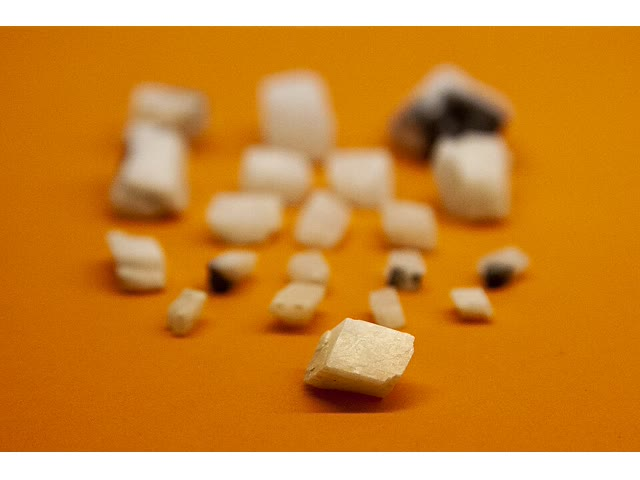
\includegraphics[width=\linewidth]{images/book3/b1-mineral-calcite-rhombs.jpg}

{\scriptsize 方解石解理菱面体。照片：Giovanna Canu 与 Eva
Santini, CC BY 4.0（维基共享资源）。}
\end{minipage}
\end{inthelab}

\begin{omfigure}
\setlength{\tabcolsep}{2pt}
\begin{tabular}{ccc}
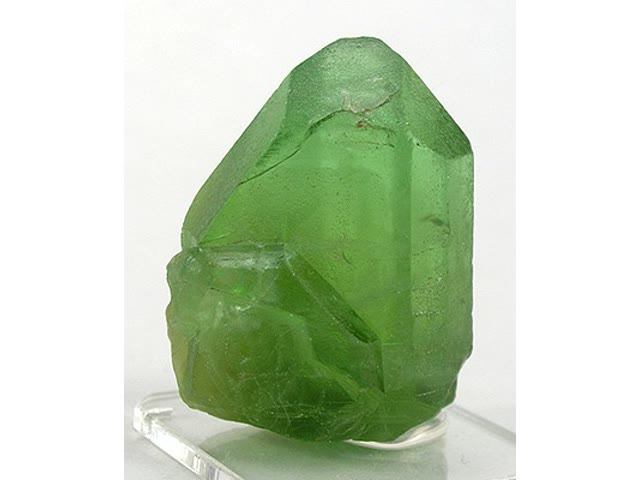
\includegraphics[width=0.31\linewidth]{images/book3/b1-mineral-olivine.jpg} &
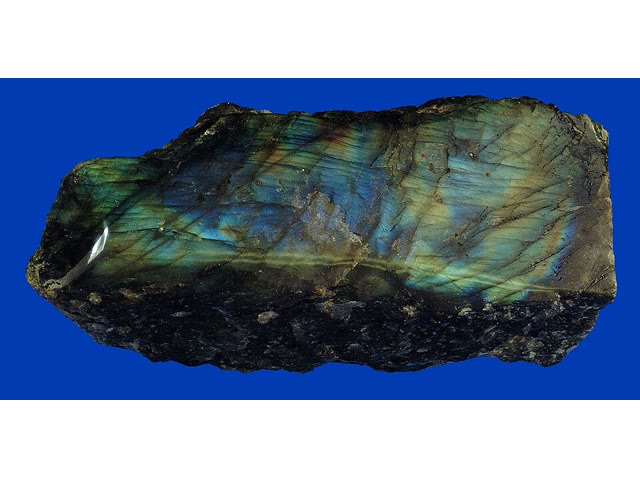
\includegraphics[width=0.31\linewidth]{images/book3/b1-mineral-plagioclase.jpg} &
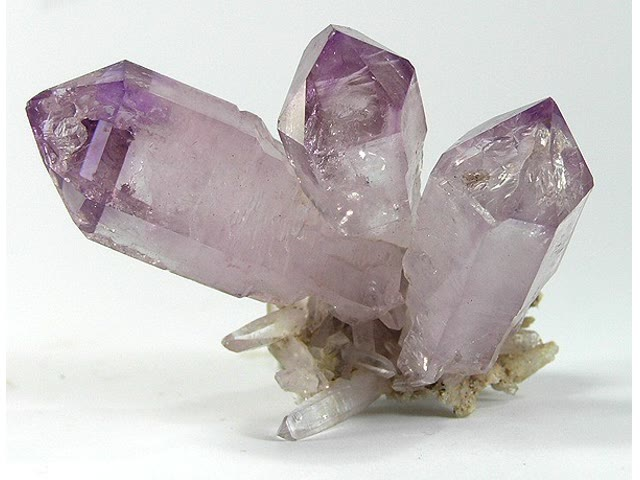
\includegraphics[width=0.31\linewidth]{images/book3/b1-mineral-quartz.jpg} \\
{\small (a) \omterm{def:b1:rock-forming-minerals:groups}{橄榄石}} & {\small (b) \omterm{def:b1:rock-forming-minerals:groups}{斜长石}（拉\omterm{def:b1:rock-forming-minerals:groups}{长石}）} & {\small (c) 石英（紫水晶）} \\[4pt]
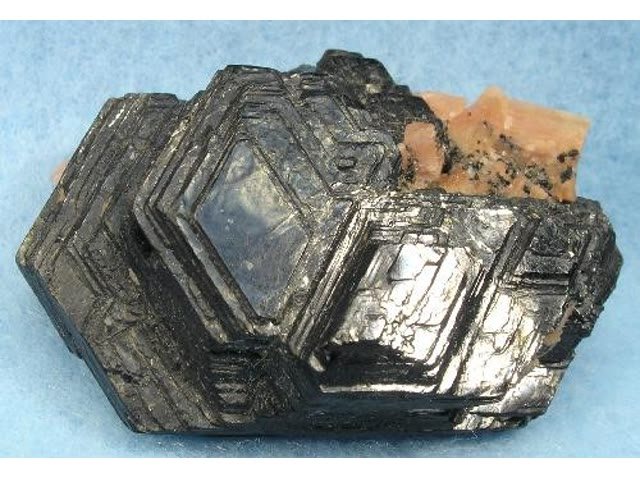
\includegraphics[width=0.31\linewidth]{images/book3/b1-mineral-biotite.jpg} &
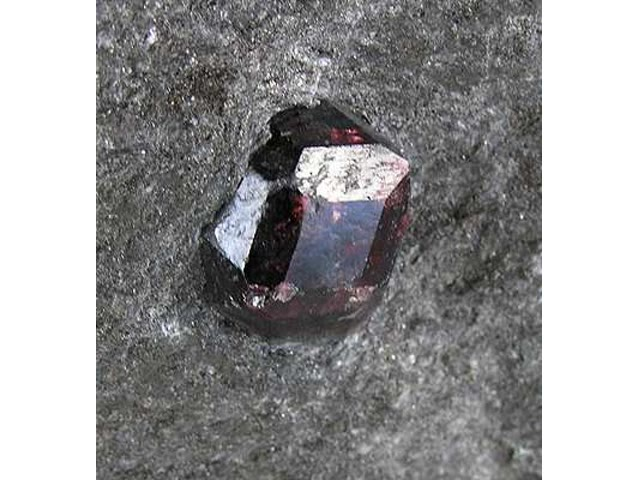
\includegraphics[width=0.31\linewidth]{images/book3/b1-mineral-garnet.jpg} &
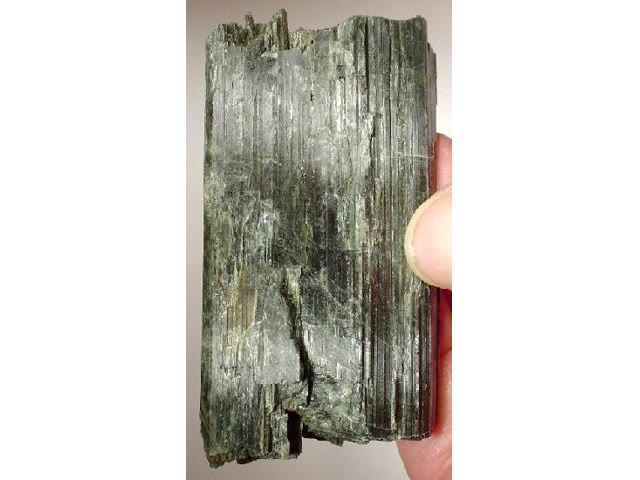
\includegraphics[width=0.31\linewidth]{images/book3/b1-mineral-hornblende.jpg} \\
{\small (d) 正\omterm{def:b1:rock-forming-minerals:groups}{长石}上的黑\omterm{def:b1:rock-forming-minerals:groups}{云母}} & {\small (e) \omterm{def:b1:rock-forming-minerals:groups}{石榴子石}（铁铝榴石）} & {\small (f) \omterm{def:b1:rock-forming-minerals:groups}{角闪石}} \\
\end{tabular}
\medskip
% ledger: commons:min-olivine, commons:min-plagioclase, commons:min-quartz, commons:min-biotite, commons:min-garnet, commons:min-hornblende

{\small 六种造岩\omterm{def:b1:rock-forming-minerals:mineral}{矿物}：(a) 宝石级\omterm{def:b1:rock-forming-minerals:groups}{橄榄石}晶体；(b) 抛光的
板片，显示拉\omterm{def:b1:rock-forming-minerals:groups}{长石}的彩色闪光；(c) 石英晶体，
六方柱状并带锥状尖端；(d) 一叠黑\omterm{def:b1:rock-forming-minerals:groups}{云母}\omterm{def:b1:field-lab-methods-1:thin-section}{薄片}，置于正\omterm{def:b1:rock-forming-minerals:groups}{长石}晶体上；
(e) 镶嵌在基质中的铁铝榴石晶体；
(f) \omterm{def:b1:rock-forming-minerals:groups}{角闪石}柱体。照片 (a)、(c)--(f) 由 Robert
M.~Lavinsky 提供，CC BY-SA 3.0；(b) 由 Twyla Baker 提供，CC0（维基共享资源）。}
\end{omfigure}

\section{练习}

\begin{exercise}[$\star$]\label{exo:b1:rock-forming-minerals:1}
指出各阴离子所属的硅酸盐类别，并给出每个四面体共用的角顶数 $s$：
\ce{SiO4^{4-}}、\ce{Si2O7^{6-}}、
\ce{Si6O18^{12-}}、\ce{Si2O5^{2-}}、\ce{SiO2}。\ce{SiO3^{2-}} 可能
属于哪一类？
\end{exercise}

\begin{exercise}[$\star$]\label{exo:b1:rock-forming-minerals:2}
取原子量 O \num{15.999}、Si \num{28.085}、Mg \num{24.305} 和
Fe \qty{55.845}{g.mol^{-1}}，计算镁\omterm{def:b1:rock-forming-minerals:groups}{橄榄石}和
铁\omterm{def:b1:rock-forming-minerals:groups}{橄榄石}的摩尔质量，再由密度 \num{3.275} 和
\qty{4.392}{g.cm^{-3}} 求出它们的摩尔体积。
% ledger: ciaaw:O, ciaaw:Si, ciaaw:Mg, ciaaw:Fe, hom:forsterite, hom:fayalite
\end{exercise}

\begin{exercise}[$\star$]\label{exo:b1:rock-forming-minerals:3}
六配位下，半径分别为 \ce{Mg^{2+}} \qty{0.72}{\angstrom}、
\ce{Fe^{2+}} \qty{0.78}{\angstrom}、\ce{Ni^{2+}} \qty{0.69}{\angstrom}、
\ce{Mn^{2+}} \qty{0.83}{\angstrom} 和 \ce{Ca^{2+}} \qty{1.00}{\angstrom}。
分别计算各离子半径与 \ce{Mg^{2+}} 半径之差，并以百分数表示，
再依据戈德施密特规则，
判断\omterm{def:b1:rock-forming-minerals:groups}{橄榄石}中哪一种离子可以自由替代镁。
% ledger: shannon:radii, goldschmidt:size
\end{exercise}

\begin{exercise}[$\star$]\label{exo:b1:rock-forming-minerals:4}
石墨和金刚石的密度分别为 \num{2.16} 和 \qty{3.51}{g.cm^{-3}}；
方解石和文石的密度分别为 \num{2.71} 和 \qty{2.93}{g.cm^{-3}}。
每一次转变中，密度各提高了百分之几？
每一对中，哪一种\omterm{def:b1:rock-forming-minerals:polymorph}{同质多象变体}在较高压强下形成？
% ledger: webmineral:polymorphs, hom:calcite
\end{exercise}

\begin{exercise}[$\star\star$]\label{exo:b1:rock-forming-minerals:5}
写出\omterm{def:b1:rock-forming-minerals:groups}{斜长石} $\text{An}_{30}$（大位上 \qty{30}{\percent}
被钙占据）的\omterm{def:b1:rock-forming-minerals:formula}{结构式}，并验证其电中性。
\end{exercise}

\begin{exercise}[$\star\star$]\label{exo:b1:rock-forming-minerals:6}
双链中，一半四面体共享两个角顶，另一半共享三个角顶。
直接在连接方式图的 (f) 图上数出四个四面体一组的重复单元中的氧原子数，
并验证化学式 \ce{Si4O11^{6-}}，
该式由\cref{prop:b1:rock-forming-minerals:si-o}给出。
\end{exercise}

\begin{exercise}[$\star\star$]\label{exo:b1:rock-forming-minerals:7}
将\omterm{def:b1:rock-forming-minerals:groups}{橄榄石}分析换算为四个氧原子基准：\qty{40.20}{\percent}
\ce{SiO2}、\qty{47.10}{\percent} \ce{MgO}、\qty{12.20}{\percent} \ce{FeO}、
\qty{0.40}{\percent} \ce{NiO}（\ce{NiO} 的摩尔质量为
\qty{74.692}{g.mol^{-1}}）。
写出其\omterm{def:b1:rock-forming-minerals:formula}{结构式}，加以验证，并给出其镁\omterm{def:b1:rock-forming-minerals:groups}{橄榄石}含量。
然后证明，仅由 \ce{MgO} 和
\ce{FeO} 的百分含量即可求出镁\omterm{def:b1:rock-forming-minerals:groups}{橄榄石}含量。
\end{exercise}

\begin{exercise}[$\star\star$]\label{exo:b1:rock-forming-minerals:8}
验证白\omterm{def:b1:rock-forming-minerals:groups}{云母} \ce{KAl2(Si3Al)O10(OH)2} 为电中性。其四面体片层
中每三个硅对应一个铝，这使每个化学式单位的片层带何种电荷，
由哪种离子来平衡它？
\end{exercise}

\begin{exercise}[$\star\star$]\label{exo:b1:rock-forming-minerals:9}
利用摩尔体积 \num{42.96} 和 \qty{46.40}{cm^3.mol^{-1}}，以及摩尔质量
\num{140.691} 和 \qty{203.771}{g.mol^{-1}}：(a) 用理想混合计算 $\text{Fo}_{50}$ 的密度，
并将其与两\omterm{def:b1:rock-forming-minerals:solid-solution}{端元}密度的平均值相比较；
(b) 求密度为
\qty{3.600}{g.cm^{-3}} 的\omterm{def:b1:rock-forming-minerals:groups}{橄榄石}的镁\omterm{def:b1:rock-forming-minerals:groups}{橄榄石}含量。
\end{exercise}

\begin{exercise}[$\star\star\star$]\label{exo:b1:rock-forming-minerals:10}
利用\cref{prop:b1:rock-forming-minerals:ideal-mixing}的记号，
证明下式成立：
\[
  \rho(x) - \bigl(x\rho_1 + (1 - x)\rho_2\bigr) =
  \frac{x(1 - x)(\rho_1 - \rho_2)(V_1 - V_2)}{V(x)} .
\]
由此推出\omterm{def:b1:rock-forming-minerals:groups}{橄榄石}的密度位于两\omterm{def:b1:rock-forming-minerals:solid-solution}{端元}之间的直线之上，
并计算 $\text{Fo}_{50}$ 处的差值。
\end{exercise}

\begin{exercise}[$\star\star\star$]\label{exo:b1:rock-forming-minerals:11}
某辉长岩中的\omterm{def:b1:rock-forming-minerals:groups}{斜长石}分析结果为 \qty{54.10}{\percent} \ce{SiO2}、
\qty{28.90}{\percent} \ce{Al2O3}、\qty{11.20}{\percent} \ce{CaO}、
\qty{5.10}{\percent} \ce{Na2O} 和 \qty{0.30}{\percent} \ce{K2O}（摩尔质量分别为
\num{60.083}、\num{101.961}、\num{56.077}、\num{61.979} 和
\qty{94.195}{g.mol^{-1}}）。换算为八个氧原子基准；检查
四面体位（Si + Al）共含 4 个原子，大位
（Ca + Na + K）共含 1 个原子；通过比较 $\mathrm{Al} - 1$ 与 Ca 验证\omterm{def:b1:rock-forming-minerals:substitution}{耦合替代}；
给出钙\omterm{def:b1:rock-forming-minerals:groups}{长石}含量 $100\,\mathrm{Ca}/(\mathrm{Ca} +
\mathrm{Na} + \mathrm{K})$。
\end{exercise}

\begin{exercise}[$\star\star\star$]\label{exo:b1:rock-forming-minerals:12}
电子探针无法区分 \ce{Fe^{2+}} 与 \ce{Fe^{3+}}，并将全部铁报告为
\ce{FeO}。(a) 证明纯磁铁矿 \ce{Fe3O4} 按此方式分析时，
总量为 \qty{93.09}{\percent}。(b) 将该分析换算为四个氧原子基准，
并说明：对于每四个氧原子含三个阳离子的\omterm{def:b1:rock-forming-minerals:mineral}{矿物}，此结果为何不可能；
(c) 改为按三个阳离子换算，并通过要求化学式电中性，
求出 \ce{Fe^{2+}} 与 \ce{Fe^{3+}} 的数目。(d) 将该分析改写为
\ce{FeO} 和 \ce{Fe2O3}，
并给出新的总量。
\end{exercise}

\section{问题：来自玄武岩的橄榄石}

\begin{problem}[{周末问题——换算橄榄石的电子探针分析，
写出并验证其化学式，并求其成分、密度，
以及一立方米玄武岩中所含的质量}]
\label{pb:b1:rock-forming-minerals:1}
% invented analysis: figdata/bachelor-1/solid_solution.py (OLIVINE_WT); values: calc/ch07.py
% ledger: ciaaw:O, ciaaw:Si, ciaaw:Mg, ciaaw:Fe, ciaaw:Mn, ciaaw:Ni, ciaaw:Ca, hom:forsterite, hom:fayalite, shannon:radii
玄武岩中绿色的晶体是\omterm{def:b1:rock-forming-minerals:groups}{橄榄石}。
对其中一颗进行电子探针分析，结果以氧化物的质量百分数表示：
\begin{center}
\small
\begin{tabular}{lcccccc}
\hline
氧化物 & \ce{SiO2} & \ce{FeO} & \ce{MnO} & \ce{MgO} & \ce{NiO} & \ce{CaO} \\
质量百分数 \% & 39.50 & 16.53 & 0.23 & 43.32 & 0.20 & 0.22 \\
\hline
\end{tabular}
\end{center}
原子量取 O \num{15.999}、Si \num{28.085}、Fe \num{55.845}、Mn
\num{54.938}、Mg \num{24.305}、Ni \num{58.693}、Ca \qty{40.078}{g.mol^{-1}}。
镁\omterm{def:b1:rock-forming-minerals:groups}{橄榄石}的密度为 \qty{3.275}{g.cm^{-3}}，铁\omterm{def:b1:rock-forming-minerals:groups}{橄榄石}的密度为
\qty{4.392}{g.cm^{-3}}。

\medskip
\noindent\textbf{第一部分——从氧化物到阳离子。}
\begin{enumerate}
  \item 计算六种氧化物的摩尔质量。
  \item 计算分析数据的总和。若总和为
        \qty{97}{\percent}，这将说明什么？
  \item 计算 \qty{100}{g} \omterm{def:b1:rock-forming-minerals:groups}{橄榄石}中每种氧化物的
        物质的量。
  \item 计算它们所含氧的物质的量及其总和。
  \item 计算每种阳离子的物质的量。
  \item 计算使氧原子数归为 4 的换算因子。
  \item 给出每 4 个氧原子对应的各元素原子数，
        保留三位小数。
\end{enumerate}

\medskip
\noindent\textbf{第二部分——\omterm{def:b1:rock-forming-minerals:formula}{结构式}。}
\begin{enumerate}[resume]
  \item 每 4 个氧原子中，\omterm{def:b1:rock-forming-minerals:groups}{橄榄石}有一个四面体间隙和
        两个八面体间隙。计算除硅以外的阳离子总和，并
        将两类间隙的总数与理想化学式比较。
  \item 写出\omterm{def:b1:rock-forming-minerals:groups}{橄榄石}的\omterm{def:b1:rock-forming-minerals:formula}{结构式}。
  \item 检验该式是否电中性，并说明为何此项检验，
        与第 8 题的检验不同，它不可能失败。
  \item 利用离子半径（\ce{Mg^{2+}} \qty{0.72}{\angstrom}，
        \ce{Fe^{2+}} \qty{0.78}{\angstrom}，\ce{Ni^{2+}}
        \qty{0.69}{\angstrom}，\ce{Mn^{2+}} \qty{0.83}{\angstrom}，
        \ce{Ca^{2+}} \qty{1.00}{\angstrom}，均为六配位），说明为何镍
        在\omterm{def:b1:rock-forming-minerals:groups}{橄榄石}中常见而钙稀少。
  \item 探针将全部铁均报告为 \ce{FeO}。请说明为何
        第 7 题中所得的阳离子总数表明\omterm{def:b1:rock-forming-minerals:groups}{橄榄石}不含
        明显的 \ce{Fe^{3+}}。
\end{enumerate}

\medskip
\noindent\textbf{第三部分——成分。}
\begin{enumerate}[resume]
  \item 计算镁\omterm{def:b1:rock-forming-minerals:groups}{橄榄石}含量 $\mathrm{Fo} = 100\,\mathrm{Mg}/(\mathrm{Mg} +
        \mathrm{Fe})$，保留一位小数。
  \item \omterm{def:b1:rock-forming-minerals:groups}{橄榄石}的 \omterm{def:b1:rock-forming-minerals:formula}{Mg 值}是多少？它在此处为何
        与镁\omterm{def:b1:rock-forming-minerals:groups}{橄榄石}含量相等？
  \item 将\omterm{def:b1:rock-forming-minerals:groups}{橄榄石}写成二元\omterm{def:b1:rock-forming-minerals:solid-solution}{固溶体}
        $\mathrm{Fo}_x\mathrm{Fa}_{1-x}$，忽略 Mn、Ni 和 Ca，并给出其
        八面体间隙中被铁占据的比例。
  \item 证明镁\omterm{def:b1:rock-forming-minerals:groups}{橄榄石}含量可仅由
        \ce{MgO} 和 \ce{FeO} 的百分含量求出，无需第 6 题的因子，
        并进行计算。
  \item 同一熔岩中后期生长的一种\omterm{def:b1:rock-forming-minerals:groups}{橄榄石}含有 \qty{40.5}{\percent}
        \ce{MgO} 和 \qty{20.0}{\percent} \ce{FeO}。计算其镁\omterm{def:b1:rock-forming-minerals:groups}{橄榄石}
        含量。哪种\omterm{def:b1:rock-forming-minerals:groups}{橄榄石}含铁更高？
\end{enumerate}

\medskip
\noindent\textbf{第四部分——密度与质量。}
\begin{enumerate}[resume]
  \item 计算镁\omterm{def:b1:rock-forming-minerals:groups}{橄榄石}和
        铁\omterm{def:b1:rock-forming-minerals:groups}{橄榄石}的摩尔质量与摩尔体积，摩尔体积保留两位小数。
  \item 将\omterm{def:b1:rock-forming-minerals:groups}{橄榄石}视为第 15 题中的二元\omterm{def:b1:rock-forming-minerals:solid-solution}{固溶体} $\mathrm{Fo}_x\mathrm{Fa}_{1-x}$，
        取 $x$ 保留三位小数，
        由理想混合计算其摩尔质量与摩尔体积。
  \item 推出其密度，保留三位小数。
  \item 将其与两\omterm{def:b1:rock-forming-minerals:solid-solution}{端元}密度之间的直线插值
        进行比较。
  \item 玄武岩中\omterm{def:b1:rock-forming-minerals:groups}{橄榄石}的体积分数为 \qty{12}{\percent}。每立方米
        玄武岩中含\omterm{def:b1:rock-forming-minerals:groups}{橄榄石}的质量为多少？
  \item 玄武岩的密度为 \qty{2.95}{g.cm^{-3}}。其中\omterm{def:b1:rock-forming-minerals:groups}{橄榄石}
        的质量分数为多少？
  \item \omterm{def:b1:rock-forming-minerals:groups}{橄榄石}的镁\omterm{def:b1:rock-forming-minerals:groups}{橄榄石}含量是多少，
        精确到整数百分比？
\end{enumerate}
\end{problem}
